\documentclass{llncs}
\newcommand{\Section}[1]{\vspace{-8pt}\section{\hskip-1em.~~#1}\vspace{-3pt}}
\newcommand{\SubSection}[1]{\vspace{-3pt}\subsection{\hskip -1em.~~#1}\vspace{-3pt}}
\newcommand{\X}{{\bf X}}
\newcommand{\x}{{\bf x}}
\newcommand{\Y}{{\bf Y}}
\newcommand{\y}{{\bf y}}
\newcommand{\Z}{{\bf Z}}
\newcommand{\z}{{\bf z}}
\newcommand{\bs}{\boldsymbol}
\newcommand{\bSigma}{\boldsymbol \Sigma}
\usepackage{amsmath,amssymb,algorithm,algorithmic}
\usepackage{times}
\usepackage{setspace,verbatim}
\usepackage{epsfig,url}
\newcommand{\argmax}{\operatornamewithlimits{argmax}}


\begin{document}
\vspace{-0.1in}
\title{Prior Constrained ROI Analysis of Brain Images}
\author{Anonymous}
\institute{Anonymous}
\maketitle              
%\vspace{-0.1in}
\begin{abstract}
 Traditionally clinicians and medical researchers have been using either totally data driven approaches like PCA/CCA/ICA or ROI based analysis for exploratory analysis of brain images. However, PCA/CCA/ICA based approaches suffer from lack of interpretability of results and on the other hand ROI based approaches are too rigid and wrongly assume that the signal lies totally within a predefined region. In this paper, we propose a novel approach which stands in stark contrast with both these approaches as it borrows strength from both these paradigms and leads to refined definitions of ROIs based on information from data. Our approach, called Prior Constrained PCA ($(PC)^2A$) provides a principled way of incorporating prior information in the form of ROIs while still allowing the data to softly modify the original ROI definitions. Experimental results on face images as well as T-1 brain images show the superiority of our approach compared to ROI and totally data based approaches.    

\end{abstract}

\section{Introduction and Related Work}
Over the last  few decades there have been significant breakthroughs in medical imaging machinery which has led to an increase in the amount and diversity of data being available e.g. structural and functional modalities, neurocognitive batteries, genetics, and environmental measurements etc. This has lead to a substantial interest in using sophisticated statistical methods to analyze and explore this data. Methods like Principal Component Analysis (PCA), Independent Component Analysis (ICA), Canonical Correlation Analysis (CCA) and their robust and sparse variants have been the workhorse of brain and neuro imaging fields as they provide key insights into the data in a totally data driven way. Particularly they find directions of maximum variance in data or its close variant and show the signal to lie in a small number of succinct regions in brain. 

However, one potential pitfall of these approaches, which has made clinicians and other researchers cautious with their use is the lack of control over the areas they highlight. Since, they work in a totally data driven way the end clinician/researcher has little control over the areas of brain they chose. Clinicians usually have some form of prior knowledge as to which areas may contain the signal they are looking for, for example, someone studying fronto-temporal dementia would expect some or most of the signal to lie in frontal cortex, however if the voxels in frontal cortex don't explain the variance in data these approaches won't highlight them. 

So, this has led the clinicians and researchers to work with totally prior driven approaches e.g. ROI (Region of Interest) analysis, where they chose a pre-defined region manually or based on past study (for instance {\em Brodmann Areas}) and study it exclusively. In other words, they wrongly assume that the entire signal is confined with in that region, i.e. frontal cortex in the above example. Though, it is not a terrible assumption that the signal lies entirely in that confined region however they are missing some important signal from data. Also, the label set might not generalize across population and different datasets as there is lots of variation in people and {\it Brodmann's} definitions might not provide the most general sets of labels.

\begin{figure*}
\begin{center}
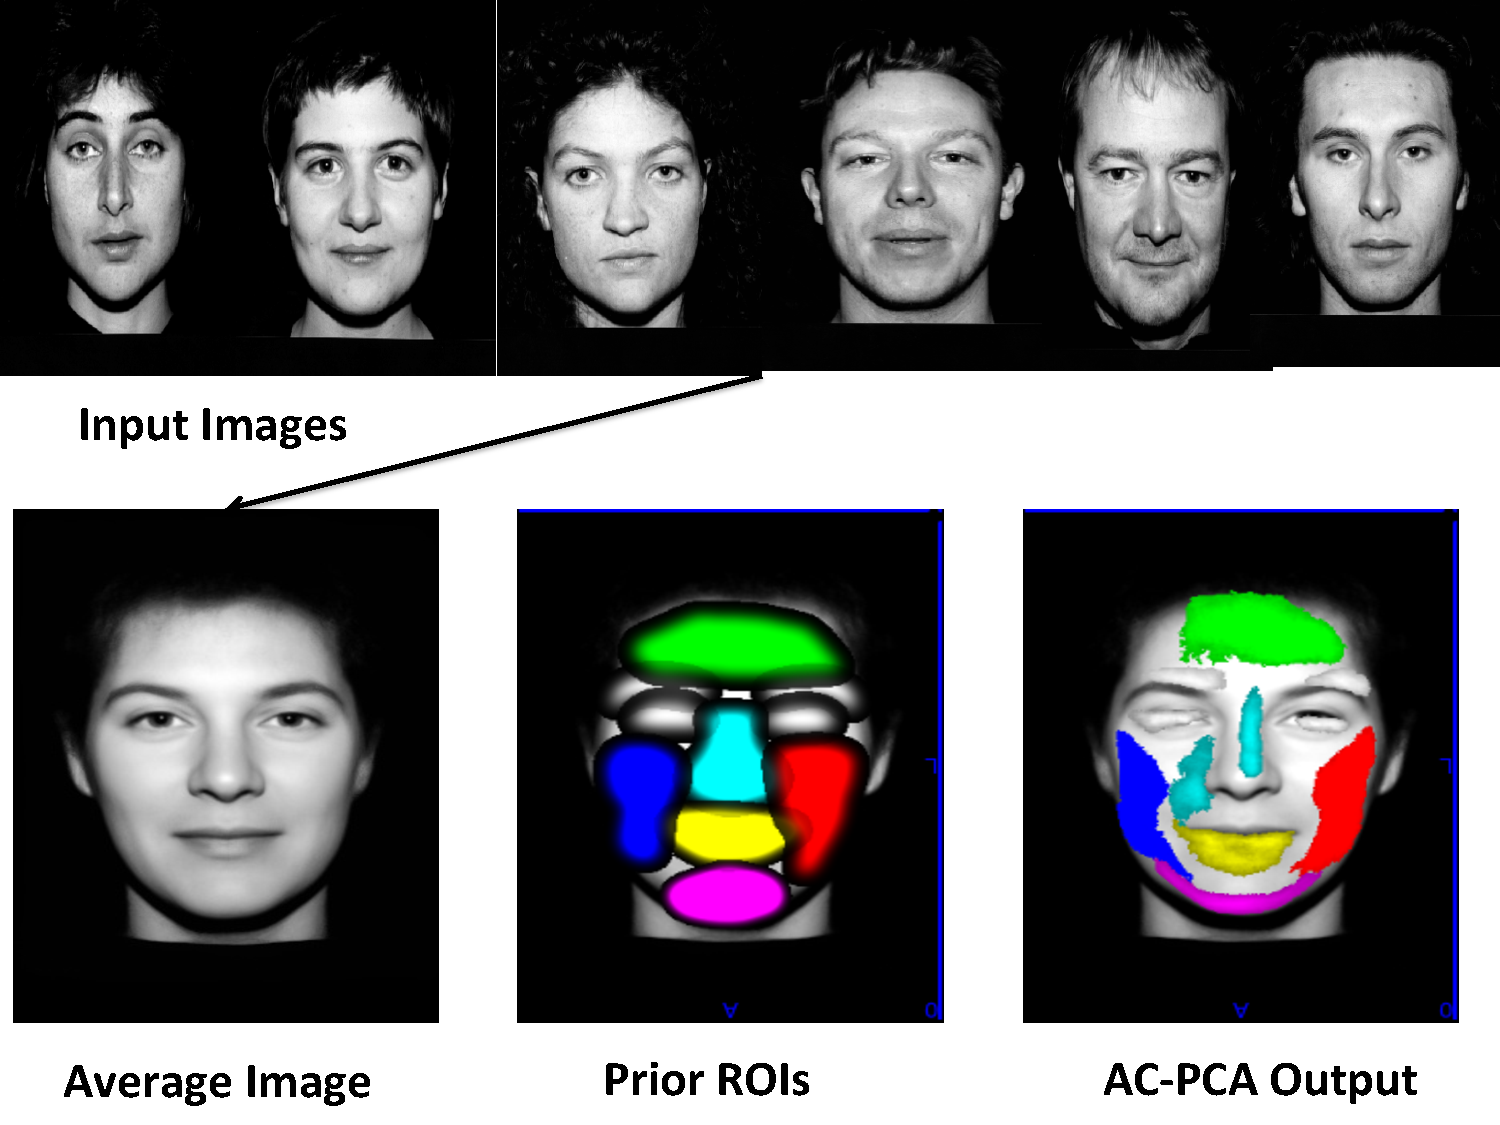
\includegraphics[width=0.7\linewidth]{fig1.pdf} 
\end{center}
\vspace{-0.2in}
\caption{$(PC)^2A$ pipeline: 1) Take in raw images 2). Register them and create an average image 3). Define Prior ROIs 4). Run $(PC)^2A$ which weighs both data and prior ROIs }
\label{fig:faces}
\end{figure*}



In this paper we propose an approach which addresses the weaknesses of both the methodologies described above, particularly, the lack of interpretability for statistical methods and wrong assumption of hard label boundaries for ROI based analysis. Our approach, called Prior Constrained PCA ($(PC)^2A$),  takes into account the neuro-anatomical variation in people while creating the ROI labels. This allows us to modify the definitions of labels to capture the variation in dataset while still staying close to the initial ROI definitions. $(PC)^2A$ provides probabilistic labels with ``soft'' boundaries and as we show in the experimental section, these ``soft'' boundaries are more sensitive to the activity in brain.

Our approach provides a principled way of incorporating priors in a totally data driven approach based on PCA. Our optimization objective provides a tradeoff between 1). staying close to the initial ROI definitions and 2). allowing data to lead the exploratory analysis by explaining variance through PCA. A good way to think about this is as ROI definitions forcing us to be {\em conservative} and staying close to the initial definitions e.g. {\it Brodmann's} areas; on the other hand the PCA component gives us {\em liberty} to be more exploratory and just trust the given data. The tradeoff between the two competing paradigms is defined by user tunable parameter, which is chosen via cross validation on a separately held validation set. Figure~\ref{fig:faces} gives an example of proof of concept of our approach using faces and also explain our general experimental pipeline used throughout this paper.


The remaining paper is organized as follows; in next section we provide the details of $(PC)^2A$ and provide an algorithm which implements our approach. In Section 3, we provide experimental results on synthetic and real datasets showing the efficacy of our approach and its superiority to both the alternatives mentioned above.


\section{ Prior Constrained Principal Component Analysis: $(PC)^2A$}
Lets assume that we are given a data matrix ${\bf X}$ where each row represents a patient (total {\bf n} of them) and each column represents a voxel in image (total {\bf p} of them). In practice, we usually have ${\bf p \gg n}$. Also, lets assume that we have a prior matrix {$\bf M(\lambda)$} (function of a parameter $lambda$ which controls its strength) whose each row corresponds to a separate prior e.g. different Brodmann areas (total {\bf k} of them) and each column (total {\bf p} of them) contains the probability of a particular voxel belonging to that prior.  

A totally data driven approach like vanilla PCA would ignore the prior matrix {\bf M} completely and just try to find combinations of voxels that explain the most variance. The objective it optimizes is:

\begin{equation}
{\bf v_i^*}= \argmax_{{\bf v_i},{\bf \|v_i\|}=1} {\bf v_i}^{\top}{\bf X^{\top}X}{\bf v_i}
\label{pca}
\end{equation}
where {$\bf v_i^*$} is the $i^{th}$ the direction of maximum variance (called eigenvector) of data matrix {\bf X}. These vectors when plotted on the image highlight regions of image which PCA (i.e. a totally data driven approach) thinks are relevant. Since, we have ${\bf p \gg n}$, the above is an ill-posed problem and we need sparsity in eigenvectors, which gives rise to Sparse PCA. The objective is exactly the same as Equation~\ref{pca} except that now we have an additional sparsity penalty ($\|\bf v \|_1$) on eigenvectors.


Our proposed algorithm $(PC)^2A$ builds on Equation~\ref{pca} and adds an additional term to the objective for incorporating prior information. Basically, it says that instead of finding the eigenvectors of the data covariance matrix (as a totally data driven approach would do), find the eigenvectors of the transformed data covariance matrix obtained by projecting it to the prior space. An important consequence of this is that we are not confining our data driven priors to lie in the original ROIs rather we are encouraging them to find ways to explain data variance but in this new ``prior projected'' space.  Also, note that instead of taking the prior as is, we smooth it as $M^s_i=\exp(\frac{M_i-1}{\lambda})$ before using it in our optimization. The modified objective is given below:
\begin{equation}
\label{ppca}
{\bf v_i^*}= \argmax_{{\bf v_i},{\bf \|v_i\|}=1} {\bf v_i}^{\top}{\bf diag(M^s_i(\lambda))}{\bf X^{\top}X}{\bf v_i} - \eta\cdot\|\bf v_i \|_1
\end{equation}
where ${\bf M^s_i(\lambda)}$ is  the ``smoothed'' the prior corresponding to the $i^{th}$ eigenvector and is itself a vector of size (${\bf 1\times p}$). The {\bf diag} operator converts the ${\bf 1\times p}$ vector into a ${\bf p\times p}$ matrix and is used just for notational convenience.  $\lambda$ is a user tunable parameter which controls the tradeoff between the influence of data and prior and should be typically tuned on a held out validation set. Its easy to see that smaller values of $\lambda$ suggest that we trust prior more and as $\lambda$ is increased we want our eigenvectors {\bf v} to be influenced more and more by the data.

Figure~\ref{fig:priorvary} shows the effect of varying the $\lambda$ parameter on the $(PC)^2A$ performance. As mentioned earlier, we choose $\lambda$ by cross-validation on a validation set.

\begin{figure*}
\begin{center}
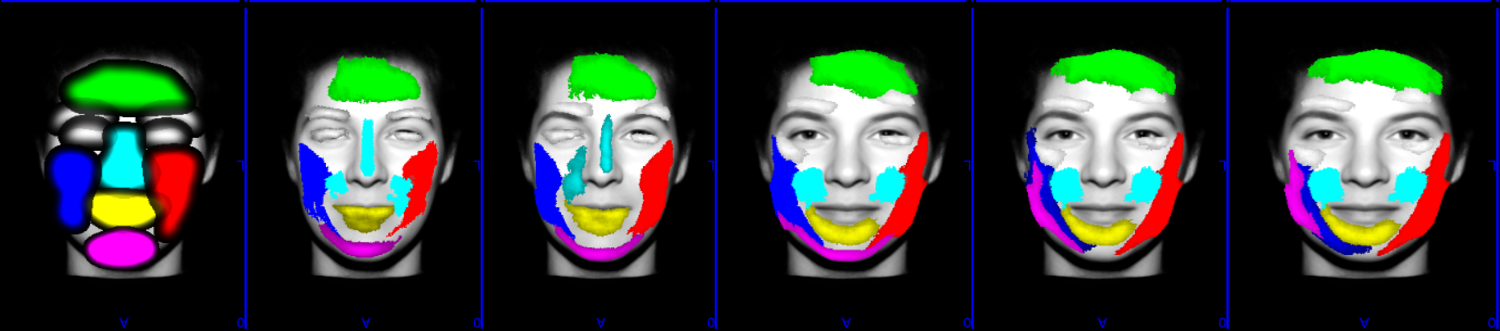
\includegraphics[width=\linewidth]{fig2.pdf} 
\end{center}
\vspace{-0.2in}
\caption{($PC)^2A$) outputs for $\lambda=[0.0,0.2,0.5,2.0,5.0,10.0]$ from left to right. Note that $\lambda =0$ corresponds to using only prior ROIs and as $\lambda$ is increased effect of data increases. This is evident from the fact that with increasing $\lambda$ our priors especially around {\em nose, eyes and eyebrows} are getting washed away.}
\label{fig:priorvary}
\end{figure*}



\subsection{An Algorithm for $(PC)^2A$}
Since our data matrices are huge, typical number of voxels in image ${\bf p}\approx 100000$, simple methods which use routines from R, MATLAB don't scale that well. Instead, we propose a fast and novel iterative algorithm in C++ (publicly available) for solving the above optimization problem. The algorithm is presented below in Algorithm~\ref{algo1}.


\begin{algorithm}[htdp]
\small \caption{\bf Prior Constrained Principal Component Analysis: $(PC)^2A$}
\label{algo1}
\begin{algorithmic}[1]
\STATE Normalize the data matrix {\bf X} by  mean centering it.
\STATE Select the (fractional) sparsity parameter $\eta$ and prior scale parameter $\lambda$
\STATE Uniformly initialize the $k$ eigenvectors $\bs v_{1,\ldots, k} \gets 1/p$ and set $j=0$.

\WHILE {$\|{\bf v_{1,\ldots,k}^{j+1}-v_{1,\ldots,k}^{j}}\|$) $<$ $\epsilon$}
\FOR {i=1 to k}
\STATE ${\bf v_i^{j}}$ $\gets$ ${\bf Xv_i^{j-1}}$ //Implements modified Arnoldi Iteration algorithm
\STATE ${\bf v_i^{j}}$ $\gets$ ${\bf X^{\top}v_i^{j}}$
\STATE ${\bf v_i^{j}}$ $\gets$ ${\bf v_i^{j}}\cdot \bf M^s_i$ // Update the eigenvector estimate with prior information.
\STATE Orthogonalize the eigenvector with respect to all other eigenvectors:\\ ${\bf v_i^{j}} \gets {\bf v_i^{j}} - \sum_{l <i} \frac{\bf v_i^{j} \bf v_l^{j}}{\bf v_l^{j} \bf v_l^{j}}  \bf v_l^{j}$
\STATE Soft-Max Sparseness:  ${\bf v_i^{j}}  \leftarrow (\|{\bf v_i^{j}}\|  - max({\bf v_i^{j}})*\eta)_+ Sign({\bf v_i^{j}})$
%\STATE Cluster Threhold: 
\STATE Normalize the eigenvector ${\bf v_i^{j}}$ $\gets$ ${\bf v_i^{j}}/\|{\bf v_i^{j}}\|$
\ENDFOR
\STATE j $\leftarrow$ j+1
\ENDWHILE
\end{algorithmic}
\end{algorithm}






%\vspace{-0.2in}
\bibliographystyle{IEEEbib}
\bibliography{./cca}

\end{document}


\text{argmax}( \x,\y) :
~\text{Corr}~( \X \x , \Y \y) - \lambda_\x \| \x \|_1 - \lambda_\y \|  \y  \|_1 , 
\end{equation} 
where $\X$ is a matrix with columns containing voxels from one set of
images of $n$ subjects, 
and $\Y$ is a matrix with columns containing voxels from the second
set of images from the same $n$ subjects. 
Corr computes Pearson correlation and the
$\lambda$ are inversely related to the sparseness costs, $C$.  %\vspace{-0.2in}

The covariance formulation of SCCA .... 

Let's compute the canonical correlation between two matrices where we
assume the matrices have been normalized and, as such, CCA computes
$$ \rho = \frac{ x \X^T \Y y  }{ \sqrt{x  \X^T \X x}\sqrt{x  \Y^T \Y y}  } $$.  Now, we change bases by
using the whitening transform.  
Redefine $\x =  ... $ Then, $\X \leftarrow \X \Sigma^{-1/2}_{XX}$ (same for $\Y$) and
$$ \rho = \frac{ x \X_w^T \Y_w \y  }{ ||x|| || y||} $$.
$$\rho = \frac{c^T \Sigma^{-1/2}_{XX} \Sigma_{XY}
  \Sigma^{-1/2}_{YY}}{\sqrt{c^Tc}\sqrt{d^Td}}$$

if matrices are whitened, then $\X \leftarrow \X \Sigma^{-1/2}_{XX}$
$$ \rho = \frac{c^T \Sigma_{XY}  d }{\sqrt{c^Tc}\sqrt{d^Td}}$$

The partial SCCA formulation will maximize 


Generally, SCCA depends upon univariate models to
factor out the effects of confounding variables.  In this paper we present a
novel algorithm for computing partial sparse canonical correlation
analysis (PSCCA) and factor (``partial'') out the effect of unwanted covariates. 

Sparse canonical correlation analysis (SCCA) is a powerful,
multivariate statistical tool for making unbiased inferences about the
relationship between different types of measurements taken on the same
population.
